
% \begin{document}

\chapter{Selective Retransmit}

Assume a client device that plays a video stream. Structurally, a video is
composed of frames, frames are then segmented into packets to stream across a
network. The client device recombines the packets into a frame and then sequences the frame to playback the video.\newline

However, the network is not-deterministic. Depending on the route the packets take
to get to the client, they may arrive out-of-order. The client may need to
maintain a receive buffer for the packets and re-order the packets back into
sequence before pushing the packets down to the decoding engine.\newline

The network may also drop packets if any of the switches along the way get busy.
In the case of a packet drop, the client has a few options. The client can
either discard the frame and let the decoding engine downstream deal with it
(which may result in visible artefacts during playback). The client can request
the whole frame to be re-sent, which results in additional bandwidth
consumption.  The client can selectively request the missing packet to be
retransmitted, which will minimize additional bandwidth consumption but increase
implementation complexity.\newline

In this chapter, we will implement a simple selective retransmit
algorithm.\newline

\begin{center}

\begin{tikzpicture}[
    packet/.style={rectangle, draw, fill=blue!20, minimum width=1cm, minimum height=0.8cm},
    missing/.style={rectangle, draw, dashed, fill=red!20, minimum width=1cm, minimum height=0.8cm},
    arrow/.style={->, >=stealth, thick}
]

    % Draw packets
    \node[packet] (p0) at (0,0) {\(pkt\ 0\)};
    \node[packet, right=0.5cm of p0] (p2) {\(pkt\ 1\)};
    \node[missing, right=0.5cm of p2] (missing1) {\(lost\)};
    \node[packet, right=0.5cm of missing1] (p4) {\(pkt\ 3\)};
    \node[packet, right=0.5cm of p4] (p5) {\(pkt\ 4\)};
    \node[right=0.5cm of p5] (dots) {\(\dots\)}; % Just dots, no box
    \node[packet, right=0.5cm of dots] (pn) {\(pkt\_n\)};

    % Draw arrows between packets
    \draw[arrow] (p0.east) -- (p2.west);
    \draw[arrow] (p2.east) -- (missing1.west);
    \draw[arrow] (missing1.east) -- (p4.west);
    \draw[arrow] (p4.east) -- (p5.west);
    \draw[arrow] (p5.east) -- (dots);
    \draw[arrow] (dots) -- (pn.west);

    % Add arrow pointing to "lost" with caption
    \draw[arrow, red] ([yshift=0.3cm] missing1.north) -- (missing1.north) 
        node[midway, above, text=red] {request to retransmit};

\end{tikzpicture}

\end{center}

Since packets may arrive out-of-order, the server stamps the packets with
sequence numbers to allow the client to order the packets as they arrive.
Once the client has a set of ordered packets, it moves the packets from the 
receive buffer into the decoding engine to be displayed.\\

The video packets are often sent via unreliable channels to minimize network
overhead and latency. The client sends an acknowledgement back to the server to
acknowledge the received packet. This indicates to the server it can send more
video data to the client. Acknowledgements are not latency-sensitive and take up
a very small proportion of bandwidth, so they are transported through reliable
channels.\\

The following illustrates packet reorder handling:
\begin{center}
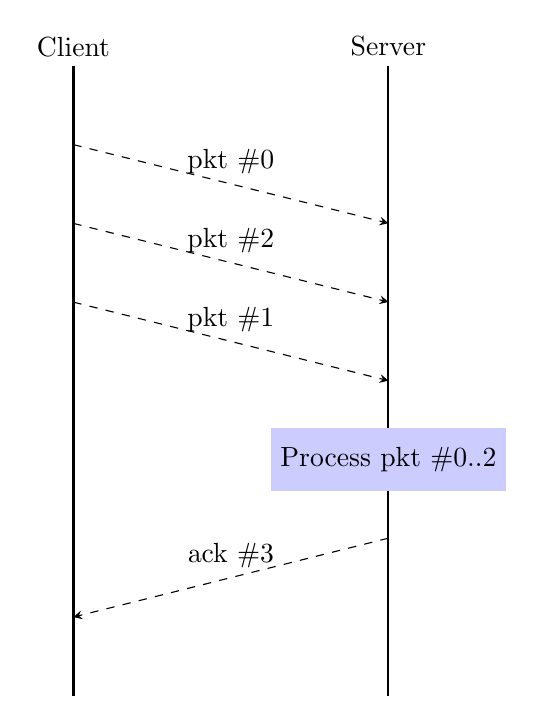
\begin{tikzpicture}[
    lifeline/.style={thick},
    message/.style={->, >=stealth, dashed},
    activation/.style={rectangle, fill=blue!20, minimum width=0.5cm, minimum height=0.8cm} ]

    \node[] (client) at (0,0) {Client};
    \node[] (server) at (4,0) {Server};

    \draw[lifeline] (client.south) -- ++(0,-8);
    \draw[lifeline] (server.south) -- ++(0,-8);

    \draw[message] ([yshift=-1cm] client.south) -- node[above] {pkt \#0} ([yshift=-2cm] server.south);
    \draw[message] ([yshift=-2cm] client.south) -- node[above] {pkt \#2} ([yshift=-3cm] server.south);
    \draw[message] ([yshift=-3cm] client.south) -- node[above] {pkt \#1} ([yshift=-4cm] server.south);
    \draw[message] ([yshift=-6cm] server.south) -- node[above] {ack \#3} ([yshift=-7cm] client.south);

    \node[activation] at ([yshift=-5cm] server.south) {Process pkt \#0..2};
\end{tikzpicture}
\end{center}

The following illustrates packet loss handling:
\begin{center}
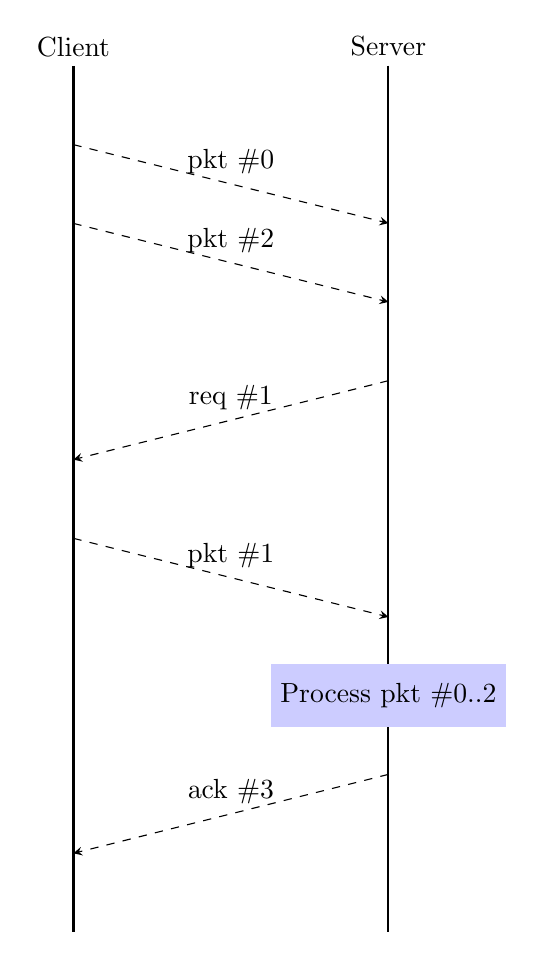
\begin{tikzpicture}[
    lifeline/.style={thick},
    message/.style={->, >=stealth, dashed},
    activation/.style={rectangle, fill=blue!20, minimum width=0.5cm, minimum height=0.8cm} ]

    \node[] (client) at (0,0) {Client};
    \node[] (server) at (4,0) {Server};

    \draw[lifeline] (client.south) -- ++(0,-11);
    \draw[lifeline] (server.south) -- ++(0,-11);

    \draw[message] ([yshift=-1cm] client.south) -- node[above] {pkt \#0} ([yshift=-2cm] server.south);
    \draw[message] ([yshift=-2cm] client.south) -- node[above] {pkt \#2} ([yshift=-3cm] server.south);
    \draw[message] ([yshift=-4cm] server.south) -- node[above] {req \#1} ([yshift=-5cm] client.south);
    \draw[message] ([yshift=-6cm] client.south) -- node[above] {pkt \#1} ([yshift=-7cm] server.south);
    \draw[message] ([yshift=-9cm] server.south) -- node[above] {ack \#3} ([yshift=-10cm] client.south);

    \node[activation] at ([yshift=-8cm] server.south) {Process pkt \#0..2};
 
\end{tikzpicture}
\end{center}

There are other design considerations. The server is allowed to send up to W
packets before getting an acknowledgement, this reduces latency perceived by the
user. The client also doesn't need to acknowledge all the packets, since the
the server assumes once an acknowledgement of packet N is received, then all packets
before N has also been received.

\section{Design}

With the above description, we are now ready to provide a more formal
description of our design:

\begin{itemize}
    \item Client is the receiver that displays the video stream.
    \item Server is the sender that sends the video stream.
    \item Server always sends the packets in order.
    \item Client may receive the packets out-of-order.
    \item Client may never receive some packet due to loss.
    \item Server can send up to W packets before an acknowledgement is received
    \item Packet sequence number is represented by a fixed number of bytes in
    the network header, the sequence number will eventually wrap around once it
    hits the maximum representable value. The maximum sequence number is
    represented as N-1. 
    \item Client puts a received packet in its receive buffer. Packets in the 
    receive buffer may be out-of-order due to network conditions.
    \item Client will remove the packets from the receive buffer once the
    sequence number of the received packets is contiguous. The client will also
    send an acknowledgement back to the Server with the most recently
    acknowledged sequence number.
    \item Data packets are transported using unreliable channels due to
    bandwidth and latency requirements.
    \item Control packets are transported using reliable channels due to relaxed 
    and latency requirements. 
\end{itemize}

We are now ready to implement the \textit{Spec}. 

\section{Spec}

The following is the skeleton of the Spec: 
\newline

\begin{tla}
Init ==
    /\ network = {}
    /\ server_tx = 0
    /\ server_tx_limit = W
    /\ server_tx_ack = 0
    /\ client_rx = 0
    /\ client_buffer = {} 
    /\ lost = 0

Next == 
    \/ Send 
    \/ \E p \in network: 
        Receive(p)
    \/ ClientRetransmitRequest
    \/ ClientAcknowledgement
    \/ \E p \in network: 
        /\ p.dst = "client" 
        /\ Drop(p)
\end{tla}
\begin{tlatex}
\@x{ Init \.{\defeq}}%
\@x{\@s{16.4} \.{\land} network \.{=} \{ \}}%
\@x{\@s{16.4} \.{\land} server\_tx \.{=} 0}%
\@x{\@s{16.4} \.{\land} server\_tx\_limit \.{=} W}%
\@x{\@s{16.4} \.{\land} server\_tx\_ack \.{=} 0}%
\@x{\@s{16.4} \.{\land} client\_rx \.{=} 0}%
\@x{\@s{16.4} \.{\land} client\_buffer \.{=} \{ \}}%
\@x{\@s{16.4} \.{\land} lost \.{=} 0}%
\@pvspace{8.0pt}%
\@x{ Next \.{\defeq}}%
\@x{\@s{16.4} \.{\lor} Send}%
\@x{\@s{16.4} \.{\lor} \E\, p \.{\in} network \.{:}}%
\@x{\@s{20.5} Receive ( p )}%
\@x{\@s{16.4} \.{\lor} ClientRetransmitRequest}%
\@x{\@s{16.4} \.{\lor} ClientAcknowledgement}%
\@x{\@s{16.4} \.{\lor} \E\, p \.{\in} network \.{:}}%
\@x{\@s{20.5} \.{\land} p . dst \.{=}\@w{client}}%
\@x{\@s{20.5} \.{\land} Drop ( p )}%
\end{tlatex}
\newline

The server is represented by three variables: 
\begin{itemize}
    \item tx+1 represents the sequence number to be used in the next packet
    \item tx\_liimit represents the highest sequence number the server can send
    without waiting for an acknowledgement
    \item tx\_ack represents the most recent acknowledged sequence number
\end{itemize}

The client is represented by two variables: 
\begin{itemize}
    \item client\_rx is the most recently acknowledged sequence number
    \item client\_buffer is the receive buffer holding all the packets waiting 
    to be re-ordered before being acknowledged\end{itemize}
The allowed actions include packet \textit{Receive}, which the existential
quantifier also has the side effect of re-ordering.
\textit{ClientRetransmitRequest} detects and sends retransmit requests.
\textit{ClientAcknowledgement} sends acknowledgement. Finally, data packets may
be dropped.\newline

Before we start defining the actions, let us define some helper functions:\newline
\begin{tla}
MinS(s) == 
    CHOOSE x \in s: \A y \in s: x <= y

MaxS(s) == 
    CHOOSE x \in s: \A y \in s: x >= y

MaxIndex == 
    LET 
        upper == {x \in client_buffer : x > N - W}
        lower == {x \in client_buffer : x < W}
        maxv == IF upper # {} /\ lower # {} 
                THEN 
                    MaxS(lower)
                ELSE 
                    MaxS(client_buffer)
    IN 
        maxv

MinIndex == 
    LET 
        upper == {x \in client_buffer : x > N - W}
        lower == {x \in client_buffer : x < W}
        minv == IF upper # {} /\ lower # {} 
                THEN 
                    MinS(upper)
                ELSE 
                    MinS(client_buffer)
    IN 
        minv

Range == 
    IF MaxIndex >= MinIndex
    THEN
        MaxIndex - MinIndex + 1
    ELSE 
        MaxIndex + 1 + N - MinIndex
\end{tla}
\begin{tlatex}
\@x{ MinS ( s ) \.{\defeq}}%
\@x{ {\CHOOSE} x \.{\in} s \.{:} \A\, y \.{\in} s \.{:} x \.{\leq} y}%
\@pvspace{8.0pt}%
\@x{ MaxS ( s ) \.{\defeq}}%
\@x{ {\CHOOSE} x \.{\in} s \.{:} \A\, y \.{\in} s \.{:} x \.{\geq} y}%
\@pvspace{8.0pt}%
\@x{ MaxIndex \.{\defeq}}%
\@x{\@s{16.4} \.{\LET}}%
 \@x{\@s{32.8} upper \.{\defeq} \{ x \.{\in} client\_buffer \.{:} x \.{>} N
 \.{-} W \}}%
 \@x{\@s{32.8} lower \.{\defeq} \{ x \.{\in} client\_buffer \.{:} x \.{<} W
 \}}%
 \@x{\@s{32.8} maxv \.{\defeq} {\IF} upper \.{\neq} \{ \} \.{\land} lower
 \.{\neq} \{ \}}%
\@x{\@s{32.8} \.{\THEN}}%
\@x{\@s{49.19} MaxS ( lower )}%
\@x{\@s{32.8} \.{\ELSE}}%
\@x{\@s{49.19} MaxS ( client\_buffer )}%
\@x{\@s{16.4} \.{\IN}}%
\@x{\@s{32.8} maxv}%
\@pvspace{8.0pt}%
\@x{ MinIndex \.{\defeq}}%
\@x{\@s{16.4} \.{\LET}}%
 \@x{\@s{32.8} upper \.{\defeq} \{ x \.{\in} client\_buffer \.{:} x \.{>} N
 \.{-} W \}}%
 \@x{\@s{32.8} lower \.{\defeq} \{ x \.{\in} client\_buffer \.{:} x \.{<} W
 \}}%
 \@x{\@s{32.8} minv \.{\defeq} {\IF} upper \.{\neq} \{ \} \.{\land} lower
 \.{\neq} \{ \}}%
\@x{\@s{32.8} \.{\THEN}}%
\@x{\@s{49.19} MinS ( upper )}%
\@x{\@s{32.8} \.{\ELSE}}%
\@x{\@s{49.19} MinS ( client\_buffer )}%
\@x{\@s{16.4} \.{\IN}}%
\@x{\@s{32.8} minv}%
\@pvspace{8.0pt}%
\@x{ Range \.{\defeq}}%
\@x{\@s{16.4} {\IF} MaxIndex \.{\geq} MinIndex}%
\@x{\@s{16.4} \.{\THEN}}%
\@x{\@s{32.8} MaxIndex \.{-} MinIndex \.{+} 1}%
\@x{\@s{16.4} \.{\ELSE}}%
\@x{\@s{32.8} MaxIndex \.{+} 1 \.{+} N \.{-} MinIndex}%
\end{tlatex}
\newline

At any moment the system allows a window of packets to be unacknowledged. Both
the client and server are aware of the window size, represented by W. By looking
at packets in its receive buffer and its most acknowledged sequence number, the
client can determine which packets were lost. There's some nuisance 
to implement this.\newline

Since the system does not allow more than W unacknowledged packets, the client
can assume the window of the packet in its receiver buffer must have sequence number
$s \in client\_rx ..client\_rx+W$. Since the sequence number has a ceiling, the
window of packets may wrap around the boundary. This introduces some
complications around determining the minimum and maximum in the window of the packet.
The functions defined above calculate the range, maximum and minimum value in
the window accounting for wraparound.\newline

Now we can look at how the client acknowledgement logic:\newline
\begin{tla}
MergeReady == 
    /\ client_buffer # {}
    /\ (client_rx + 1) % N = MinIndex       \* contiguous with previous ack
    /\ Range = Cardinality(client_buffer)   \* combined is contiguous 

ClientAcknowledgement == 
    /\ client_buffer # {}
    /\ MergeReady 
    /\ client_buffer' = {}
    /\ client_rx' = MaxIndex
    /\ network' = AddMessage([dst |-> "server",
                              type |-> "ack",
                              ack |-> MaxIndex], 
                                network)
    /\ UNCHANGED <<server_tx, server_tx_ack, server_tx_limit, lost>>
\end{tla}
\begin{tlatex}
\@x{ MergeReady \.{\defeq}}%
\@x{\@s{16.4} \.{\land} client\_buffer \.{\neq} \{ \}}%
 \@x{\@s{16.4} \.{\land} ( client\_rx \.{+} 1 ) \.{\%} N \.{=}
 MinIndex\@s{24.59}}%
\@y{%
  contiguous with previous ack
}%
\@xx{}%
\@x{\@s{16.4} \.{\land} Range \.{=} Cardinality ( client\_buffer )\@s{24.6}}%
\@y{%
  combined is contiguous 
}%
\@xx{}%
\@pvspace{8.0pt}%
\@x{ ClientAcknowledgement \.{\defeq}}%
\@x{\@s{16.4} \.{\land} client\_buffer \.{\neq} \{ \}}%
\@x{\@s{16.4} \.{\land} MergeReady}%
\@x{\@s{16.4} \.{\land} client\_buffer \.{'} \.{=} \{ \}}%
\@x{\@s{16.4} \.{\land} client\_rx \.{'} \.{=} MaxIndex}%
 \@x{\@s{16.4} \.{\land} network \.{'} \.{=} AddMessage ( [ dst
 \.{\mapsto}\@w{server} ,\,}%
\@x{\@s{16.4} type \.{\mapsto}\@w{ack} ,\,}%
\@x{\@s{16.4} ack \.{\mapsto} MaxIndex ] ,\,}%
\@x{\@s{24.59} network )}%
 \@x{\@s{16.4} \.{\land} {\UNCHANGED} {\langle} server\_tx ,\, server\_tx\_ack
 ,\, server\_tx\_limit ,\, lost {\rangle}}%
\end{tlatex}
\newline

The client only acknowledges when it has a contiguous sequence of packets that
follows its most recently acknowledged packet. When MergeReady is true, the
client sends the acknowledgement back to the server.\newline

\begin{tla}
ClientReceive(pp) == 
    /\ network' = RemoveMessage(pp, network)
    /\ client_buffer' = client_buffer \cup {pp.seq}
    /\ UNCHANGED <<server_tx, client_rx, 
        server_tx_ack, server_tx_limit, lost>>

Missing == 
    LET 
        full_seq == 
            IF MaxIndex >= client_rx+1 
            THEN 
                {x \in client_rx+1 .. MaxIndex : TRUE}
            ELSE 
                {x \in 0..MaxIndex : TRUE} \cup {x \in client_rx + 1..N-1 : TRUE}
        all_client_msgs == {m \in network: m.dst = "client"}
        all_client_seqs == {m.seq : m \in all_client_msgs}
        network_missing == full_seq \ all_client_seqs
        client_missing == full_seq \ client_buffer
        to_request == network_missing \intersect client_missing
    IN 
        to_request

ClientRetransmitRequest == 
    /\ ~MergeReady
    /\ client_buffer # {}
    /\ Missing # {}
    /\ network' = AddMessage([dst |-> "server", 
                              type |-> "retransmit",
                              seq |-> CHOOSE x \in Missing : TRUE],
                                network)
    /\ UNCHANGED <<server_tx, server_tx_limit, 
        client_rx, client_buffer, server_tx_ack, lost>>
\end{tla}
\begin{tlatex}
\@x{ ClientReceive ( pp ) \.{\defeq}}%
\@x{\@s{16.4} \.{\land} network \.{'} \.{=} RemoveMessage ( pp ,\, network )}%
 \@x{\@s{16.4} \.{\land} client\_buffer \.{'} \.{=} client\_buffer \.{\cup} \{
 pp . seq \}}%
\@x{\@s{16.4} \.{\land} {\UNCHANGED} {\langle} server\_tx ,\, client\_rx ,\,}%
\@x{\@s{20.5} server\_tx\_ack ,\, server\_tx\_limit ,\, lost {\rangle}}%
\@pvspace{8.0pt}%
\@x{ Missing \.{\defeq}}%
\@x{\@s{16.4} \.{\LET}}%
\@x{\@s{32.8} full\_seq \.{\defeq}}%
\@x{\@s{49.19} {\IF} MaxIndex \.{\geq} client\_rx \.{+} 1}%
\@x{\@s{49.19} \.{\THEN}}%
 \@x{\@s{65.6} \{ x \.{\in} client\_rx \.{+} 1 \.{\dotdot} MaxIndex \.{:}
 {\TRUE} \}}%
\@x{\@s{49.19} \.{\ELSE}}%
 \@x{\@s{65.6} \{ x \.{\in} 0 \.{\dotdot} MaxIndex \.{:} {\TRUE} \} \.{\cup}
 \{ x \.{\in} client\_rx \.{+} 1 \.{\dotdot} N \.{-} 1 \.{:} {\TRUE} \}}%
 \@x{\@s{32.8} all\_client\_msgs \.{\defeq} \{ m \.{\in} network \.{:} m . dst
 \.{=}\@w{client} \}}%
 \@x{\@s{32.8} all\_client\_seqs \.{\defeq} \{ m . seq \.{:} m \.{\in}
 all\_client\_msgs \}}%
 \@x{\@s{32.8} network\_missing \.{\defeq} full\_seq \.{\,\backslash\,}
 all\_client\_seqs}%
 \@x{\@s{32.8} client\_missing \.{\defeq} full\_seq \.{\,\backslash\,}
 client\_buffer}%
 \@x{\@s{32.8} to\_request \.{\defeq} network\_missing \.{\cap}
 client\_missing}%
\@x{\@s{16.4} \.{\IN}}%
\@x{\@s{32.8} to\_request}%
\@pvspace{8.0pt}%
\@x{ ClientRetransmitRequest \.{\defeq}}%
\@x{\@s{16.4} \.{\land} {\lnot} MergeReady}%
\@x{\@s{16.4} \.{\land} client\_buffer \.{\neq} \{ \}}%
\@x{\@s{16.4} \.{\land} Missing \.{\neq} \{ \}}%
 \@x{\@s{16.4} \.{\land} network \.{'} \.{=} AddMessage ( [ dst
 \.{\mapsto}\@w{server} ,\,}%
\@x{\@s{16.4} type \.{\mapsto}\@w{retransmit} ,\,}%
 \@x{\@s{16.4} seq \.{\mapsto} {\CHOOSE} x \.{\in} Missing \.{:} {\TRUE} ]
 ,\,}%
\@x{\@s{24.59} network )}%
 \@x{\@s{16.4} \.{\land} {\UNCHANGED} {\langle} server\_tx ,\,
 server\_tx\_limit ,\,}%
 \@x{\@s{20.5} client\_rx ,\, client\_buffer ,\, server\_tx\_ack ,\, lost
 {\rangle}}%
\end{tlatex}
\newline

\textit{ClientReceive} moves the packet from the network into the client receive
buffer. The only reason why this is done as a separate step is to make debugging
easier.\newline

\textit{Missing} returns a set of missing missing sequence numbers. This is done
by cross-checking the client receive buffer and the outstanding network packet
targeting the client. In theory, the client doesn't know if a gap in its receive
buffer means the packet is lost or will arrive soon. Practically, the client
will assume a packet is lost after some configurable timeout and request a
retransmit.\newline

Let us take a look at server-related definitions:\newline

\begin{tla}
RemoveStaleAck(ack, msgs) == 
    LET 
        acks == {(ack - k + N ) % N : k \in 1..W}
    IN 
        {m \in msgs : ~(/\ m.dst = "server" 
                        /\ m.type = "ack" 
                        /\ m.ack \in acks)}

ServerReceive(pp) == 
    \/ /\ pp.type = "ack"
       /\ server_tx_ack' = pp.ack
       /\ server_tx_limit' = (pp.ack + W) % N
       /\ network' = RemoveStaleAck(pp.ack, RemoveMessage(pp, network))
       /\ UNCHANGED <<server_tx, client_rx, client_buffer, lost>>
    \/ /\ pp.type = "retransmit"
       /\ network' = AddMessage([dst |-> "client", seq |-> pp.seq], 
                                RemoveMessage(pp, network))
       /\ lost' = lost -1
       /\ UNCHANGED <<server_tx, server_tx_limit, 
            client_rx, client_buffer, server_tx_ack>>
\end{tla}
\begin{tlatex}
\@x{ RemoveStaleAck ( ack ,\, msgs ) \.{\defeq}}%
\@x{\@s{16.4} \.{\LET}}%
 \@x{\@s{32.8} acks \.{\defeq} \{ ( ack \.{-} k \.{+} N ) \.{\%} N \.{:} k
 \.{\in} 1 \.{\dotdot} W \}}%
\@x{\@s{16.4} \.{\IN}}%
 \@x{\@s{32.8} \{ m \.{\in} msgs \.{:} {\lnot} ( \.{\land} m . dst
 \.{=}\@w{server}}%
\@x{\@s{36.89} \.{\land} m . type \.{=}\@w{ack}}%
\@x{\@s{36.89} \.{\land} m . ack \.{\in} acks ) \}}%
\@pvspace{8.0pt}%
\@x{ ServerReceive ( pp ) \.{\defeq}}%
\@x{\@s{16.4} \.{\lor} \.{\land} pp . type \.{=}\@w{ack}}%
\@x{\@s{16.4} \.{\land} server\_tx\_ack \.{'} \.{=} pp . ack}%
 \@x{\@s{16.4} \.{\land} server\_tx\_limit \.{'} \.{=} ( pp . ack \.{+} W )
 \.{\%} N}%
 \@x{\@s{16.4} \.{\land} network \.{'} \.{=} RemoveStaleAck ( pp . ack ,\,
 RemoveMessage ( pp ,\, network ) )}%
 \@x{\@s{16.4} \.{\land} {\UNCHANGED} {\langle} server\_tx ,\, client\_rx ,\,
 client\_buffer ,\, lost {\rangle}}%
\@x{\@s{16.4} \.{\lor} \.{\land} pp . type \.{=}\@w{retransmit}}%
 \@x{\@s{16.4} \.{\land} network \.{'} \.{=} AddMessage ( [ dst
 \.{\mapsto}\@w{client} ,\, seq \.{\mapsto} pp . seq ] ,\,}%
\@x{\@s{16.4} RemoveMessage ( pp ,\, network ) )}%
\@x{\@s{16.4} \.{\land} lost \.{'} \.{=} lost \.{-} 1}%
 \@x{\@s{16.4} \.{\land} {\UNCHANGED} {\langle} server\_tx ,\,
 server\_tx\_limit ,\,}%
\@x{\@s{24.59} client\_rx ,\, client\_buffer ,\, server\_tx\_ack {\rangle}}%
\end{tlatex}
\newline

When the server receives an acknowledgement for sequence number K, it assumes
K-1 and prior were all received by the client. \textit{RemoveStaleAck} is a
model optimization to drop all acknowledgements with sequence numbers less than
K. Note that sequence numbers k, k-N, and k-2*N, are all represented as k, and
intheory, the client may not be able to differentiate between them.
Practically, N is sized large enough to represent a few second's worth of data,
so the system can safely assume a sequence number k is for the most recent N
packets.\\

Upon receiving an acknowledgement from the client, the server bumps the
server\_tx\_limit allowing it to send more data. The server can also receive a 
retransmit request and send the requested data. \textit{lost} is configurable to
determine how many packets can be dropped at the same time.

\section{Refinement}

\subsection{Removing Stale Acknowlegement}

When the server acknowledges K, it has already received all the packets before
K. Likewise, when the client receives an acknowledgement for K, it can assume
all previous packets have been received. The client may receive the
acknowledgement out-of-order due to unfavourable network conditions. One
refinement we can make to the model is simply \textit{remove all stale
acknowledgements}. In a practical implementation, this is also how the client
can react when it receives stale acknowledgements.\\

There is a bit of nuisance here. Since the sequence number wraps around, the
client cannot differentiate between K from K-N, K-2*N, etc. However, N
is usually large enough to accommodate a few seconds of data before a sequence
number is re-used. The client can be confident that any K received the current
K, not K-N or earlier.

\subsection{Retransmit Request Assumed Reliable}

Retransmit requests packets can be delivered through unreliable channels. However,
this makes no difference in the model. The client sends a retransmit request
when it detects packets are lost. If the model drops the retransmit request, the
client will just send another retransmit request because the missing packet is
still missing.\\

While this can be modeled, it would increase the runtime without providing many
benefits. For this Spec, we simply assume all control packets are reliable. 

\section{Safety}

\section{Liveness}

Given the system may randomly drop packets, one possible liveness condition is
to verify packets of all sequence numbers are received by the client at some
point. This can be described as for all possible sequence number value k, k is
eventually exists in the client receive buffer.\\

\begin{tla}
Liveness == 
    \A i \in 0..N-1:
        client_buffer = {} ~> \E j \in client_buffer: i = j 
\end{tla}
\begin{tlatex}
\@x{ Liveness \.{\defeq}}%
\@x{\@s{16.4} \A\, i \.{\in} 0 \.{\dotdot} N \.{-} 1 \.{:}}%
 \@x{\@s{20.5} client\_buffer \.{=} \{ \} \.{\leadsto} \E\, j \.{\in}
 client\_buffer \.{:} i \.{=} j}%
\end{tlatex}

% \end{document}
